\begin{figure}[H]
\centering
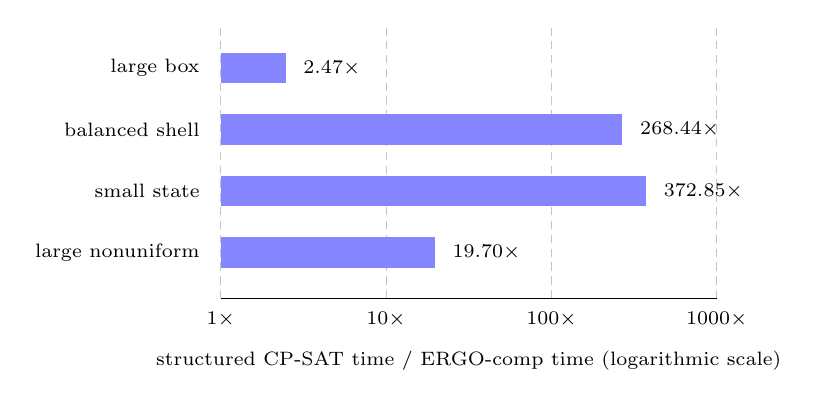
\begin{tikzpicture}[x=2.1cm,y=0.78cm]
  \scriptsize
  \foreach \x/\lab in {0/{1},1/{10},2/{100},3/{1000}} {
    \draw[gray!45, densely dashed] (\x,0.25) -- (\x,4.65);
    \node[below] at (\x,0.15) {$\lab\times$};
  }
  \draw[semithick] (0,0.25) -- (3,0.25);
  \foreach \y/\name/\w/\value in {
    4/{large box}/0.392/{2.47\times},
    3/{balanced shell}/2.429/{268.44\times},
    2/{small state}/2.572/{372.85\times},
    1/{large nonuniform}/1.294/{19.70\times}} {
    \node[anchor=east] at (-0.08,\y) {\name};
    \fill[blue!48] (0,\y-0.25) rectangle (\w,\y+0.25);
    \node[anchor=west, font=\scriptsize\bfseries] at (\w+0.06,\y) {$\value$};
  }
  \node[below] at (1.5,-0.48) {structured CP-SAT time / ERGO-comp time (logarithmic scale)};
\end{tikzpicture}
\caption{ERGO-comp speedup over structured CP-SAT on the four recorded exact
scheduler profiles.  Both solvers receive the same safe preprocessing and must
return the same optimum and retained loads.  The bars summarize the exact
medians in Table~\ref{tab:ergo-comp-cpsat}; they are bounded implementation
measurements, not a general solver ranking.}
\label{fig:ergo-comp-cpsat}
\end{figure}
